\documentclass{sig-alternate}
%\documentclass{sig-alternate-10pt}
 
\usepackage{verbatim}
\usepackage{graphics}
\usepackage{color}
\usepackage{url}
\usepackage{subfigure}
\usepackage{mdwlist}
\usepackage{floatflt}
\usepackage{pgfplots}
%\pgfplotsset{compat=1.3}
\pgfplotsset{every axis/.append style={
                    legend style={mark size=4pt},
                    }}

\begin{document}

\conferenceinfo{ExtremeCom}{2014}
\CopyrightYear
\crdata

\title{The Breadcrumb Router: Bundle Trajectory Tracking and Geographic Source Routing in DTN
\thanks{\hrule\vspace{0.1in} This work was funded in part by the Laboratory
for Telecommunications Sciences, US Department of Defense.  The opinions
expressed in this paper reflect those of the authors, and do not
necessarily represent those of the Department of Defense or US Federal
Government.}}

\author{
\alignauthor
Tomasz Kalbarczyk\textsuperscript{\#}\quad Brenton
Walker\textsuperscript{*}\quad Christine
Julien\textsuperscript{\#}\quad Angela
Hennessy\textsuperscript{*}\quad\\
Pedro
Santacruz\textsuperscript{\#}\quad Jonas Michel\textsuperscript{\#}\quad Amy
Alford\textsuperscript{\$}\quad \\  
\affaddr{\textsuperscript{\#}The University of Texas at Austin,
Austin, TX}\\
Email: \{tkalbar, pesantacruz, jonasrmichel, c.julien\}@utexas.edu\\
\affaddr{\textsuperscript{*}Laboratory for Telecommunications
Sciences, College Park, MD}\\
Email: brenton@ltsnet.net, ahennes1@math.umd.edu\\
\affaddr{\textsuperscript{\$}The University of Maryland, College Park,
MD}\\
Email: aloomis@math.umd.edu
}


%\numberofauthors{4} 
%\author{
%% 1st. author
%\alignauthor
%Tomasz Kalbarczyk, Pedro Santacruz, Jonas Michel, and Christine Julien\\
%       \affaddr{University of Texas-Austin}\\
%      \email{\{tkalbar, pesantacruz, jonasrmichel, c.julien\}@utexas.edu}
%% 2nd author
%\alignauthor
%Brenton Walker and Angela Hennessy\\
%       \affaddr{Laboratory for Telecommunications Sciences}\\
%       \affaddr{College Park, MD, USA}\\
%       \email{\{brenton, calvin\}@ltsnet.net}
%% 3rd author
%\alignauthor
%Amy Alford\\
%       \affaddr{University of Maryland}\\
%       \affaddr{College Park, MD, USA}\\
%       \email{aloomis@math.umd.edu}
%}

\maketitle

\begin{abstract}
\begin{sloppypar}
Since the dawn of time, man has wanted to know where the heck his bundles went, and to send them back on a specific geo-coded route.  Our new BreadCrumb Router and its associated extension block processors satisfiy this cosmic desire of human existence.  
\end{sloppypar}
\end{abstract}

\category{C.2.1}{Network Architecture and Design}{Store and forward networks}
%\terms{Design, Experimentation, Performance}
\keywords{Delay-tolerant networks, bundle protocol, geographic routing}

% -----------------------------------------------
%
%   Introduction
%
% -----------------------------------------------
\section{Introduction}
Applications in delay-tolerant networks (DTNs) often desire to both track the path(s) of data through the network and to directly influence the movement of the data. DTNs are almost always integrated into some physical space that also influences that movement of nodes, data, and the phenomena about which the nodes communicate. In traditional IP networks, the {\bf traceroute} tool and {\bf source routing} protocols have assisted in {\em tracking} and {\em directing} packets of data, but the focus has traditionally been on movement through the logical network and not through physical space.

When the physical and logical intertwine, there is a desire for data movement to reflect various aspects of the physical space the data inhabits. We address the dual challenges of {\em tracking} data as it moves through space and time and intentionally {\em routing} data through space and time. As an exemplar of tracking, consider the need for {\em data provenance} in sensing aggregation. As an aggregate collects information sensed about a physical phenomenon, the aggregate may need to dynamically compute the data {\em coverage} by tracking where the aggregate has traveled and collected information~\cite{michel12:spatiotemporal}. As an exemplar of the routing challenge, consider a piece of data that measures the concentration of a gas leak. Users in the area where the gas is expected to dissipate should be warned; this can be accomplished by associating the data item with a route through space and time that captures this expected dissipation. Tracking and routing can also be combined; imagine a generic scenario in which a {\em publisher} generates a piece of data that tracks its movement {\em en route} to a {\em subscriber}. Upon receiving the publication, the subscriber sends a response that must follow the reverse path of the original publication. This generic situation is a stand-in for a variety of concrete applications. For example, the original publication may have reserved some resources along the routing path that the return response relies on. In the later sections of this paper, we use a concrete story behind this more general scenario. Specifically, we consider a maze traversal in which a prisoner in the maze sends a probe that tracks its path as it attempts to exit the maze. When it reaches the exit, the responder (e.g. a rescuer) sends a response packet back to the prisoner along the same path through the maze.

Our problem of tracking differs substantially from the goals of existing utilities, not only in terms of the transition from logical network hops to physical spaces but also because the route a bundle in a DTN takes may not be stable (one bundle may pass through a given sequence of nodes, while a bundle sent just a minute later may take a different route). It therefore may often be important to track the route of {\em each} bundle. In our tracking facility, we track {\em both} logical network hops and the sequence of geographic locations it visits (whether because a device at one location transmits the bundle to a device at a different location or because the device holding the bundle moves). Besides being an illuminating diagnostic tool to understand the behavior of a DTN, tracking a bundle's geographic route can capture important meta-information related to the bundle's contents, as motivated above. 

Source routing, in which a packet carries with it the specific network hops it must traverse, and geographic routing, where packet routing is based on physical locations, have been popular in mobile ad hoc networks~\cite{johnson96:dynamic, karp00:gpsr}. We combine these approaches into a geographically informed version of source routing. Previous approaches to geographic routing predominantly use a {\em greedy} approach in which locally optimal decisions are used to move a bundle incrementally closer to its destination. Our approach to {\em geo-source routing} differs in that it allows the sender to pre-specify a sequence of geo-locations that serve as routing {\em waypoints}. This style of approach can solve a variety of challenges associated with traditional geographic routing. For example by explicitly directing the geographic path of a bundle, our protocol can explicitly route around known dead-ends in the network or around known areas of congestion in the network. Combining this style of geo-routing with other approaches could, for example, ensure that network coded bundles~\cite{petz11:network, widmer05:network} take sufficiently diverse routes through the network.

We introduce the {\sc breadcrumb} router, which implements geo-source routing on DTN bundles that can pre-specify their own delivery paths by providing a combination of geo-locations and logical network hops. 
%In our {\sc breadcrumb} router, elements in this sequence can be {\em required}, meaning that the bundle must touch the specified logical or physical location or {\em optional}, meaning that the sequence serves as a suggestion that the {\sc breadcrumb} router can use simply to guide its decision making. 
Each geo-location comes with a {\em margin of error}, which allows the bundle to get {\em near} the specified location without having to exactly reach it. We also introduce two bundle {\em extension blocks}. The {\em GeoRouting} block holds the sequence of logical and geographical waypoints for geo-source routing. The {\em GeoTracking} block allows any bundle to collect a sequence of locations it visits in both logical and physical space. In our implementation, we rely on a GPS module to provide location information. Throughout the paper, we use the phrases ``GPS location'' or ``GPS coordinates'' to refer to this information, but we note that the GPS framework is a stand-in for any available, potentially highly fine-grained location service framework.  We describe our the {\sc breadcrumb} router and the two extension blocks conceptually and show how we have implemented them in the IBR-DTN implementation of the bundle routing protocol~\cite{IBR-DTN-WASA}. We connect the {\sc breadcrumb} router to our existing Java-based implementation of {\em spatiotemporal trajectories}~\cite{michel12:spatiotemporal}, in which applications can perform expressive computations over data items given knowledge of their movements in space and time and geo-tracking and geo-routing of bundles on a pair of mobility scenarios.



%{\color{blue}
%Since the dawn of time, man has wanted to know where the heck his bundles went, and to send them back on a specific geo-coded route.  Our new BreadCrumb Router and its associated extension block processors satisfy this cosmic desire of human existence.  

%The {\bf traceroute} tool is a staple of traditional IP networks.  It allows a user or administrator to discover the sequence of IP routers their packets pass through between a specific source and destination.  Traceroute works by taking advantage of existing IGMP hop-count and reporting requirements.  Bundle Protocol as defined in RFC5050 has no inherent facility that can achieve this.  Furthermore, because the route a bundle takes may not be stable (one bundle may pass through one sequence of nodes, and a bundle sent a minute later may take another route) it is more salient in a DTN to comprehensively track the entire route of a single bundle, rather than send a series of bundles to probe the network.  Therefore bundle tracking functionality must be built fully as an extension to BP.  Additionally, since in many use cases the geographic mobility of the nodes in a DTN plays an integral part in the routing and delivery of a bundle, tracking the geographic route a bundle follows can be at least as interesting, and possibly {\it more} salient than the logical hops the bundle passes through.

%Besides being an illuminating diagnostic tool to understand the behavior of a DTN, tracking the geographic route of a bundle can capture important meta-information related to the contents of a bundle.  The simplest example of this is simply geo-tagging the location where a bundle originated.  A more involved example is tinkerpopping the datums of an oil slick with trajectories with a graph database as described in \cite{jonas-paper} and to be elaborated on here and in the following sections by Jonas and Christine.  Datums: it's the plural of ``datum'' when you're talking about geodetic information, dammit!

%Converse to simply geotracking a bundle, we build a prototype router for source geo-routing of a bundle.  In traditional IP networks, extensions to support source routing are defined for both IPv4 and IPv6, but are rarely used and often not supported or blocked.  On the other hand source routing is an integral part of some MANET routing protocols \cite{some-DSR-paper}.  Some reasons source routing could be used are to probe the structure of a network, or to specify that packets should avoid sections of a network that are known to be problematic because of congestion, reliability, or security concerns.  Implementing this type of {\it logical} hop-based source routing in DTN is certainly feasible, but in a dynamic mobile network is is difficult to imagine that a source will know exactly which intermediate nodes will be available to ferry its bundles.  Considering the importance of the geographic path in DTN routing, we propose geographic source routing.  In this system a sender can specify both logical (intermediate nodes) and geographic waypoints a bundle must pass through on its way to the destination.

%Geographic routing has been proposed and used in many DTN scenarios \cite{paper1,paper2,paper3,paper4,paper5,paper6}.  In most cases greedy geographic routing is used locally to move a bundle closer to a destination.  In other cases large-scale logical hops over an infrastructure network are used to get a bundle to a general geographic area of interest, and then other types of routing take precedence to get the bundle to its final destination.  Source geo-routing is different in that it allows a sender to pre-specify solutions to problems that can arise from greedy geographic routing.  Some of these issues and goals are:
%\begin{itemize}
%  \item avoiding known dead-ends in the network. I.e. local minima in the greedy geographic routing heuristic.
%  \item avoiding geographic areas where unreliability or congestion is anticipated.  For example if a shortest geographic route goes past a baseball stadium, but a game is scheduled for that day, a source may request that a bundle be routed around the expected traffic jam.
%  \item ensuring that network coded bundles take sufficiently diverse routes.  Since network coded information can be viewed as a shared secret problem, ensuring that not all of the encodings are ever in the same geographic area could be a security measure in a DTN.
%\end{itemize}
%\footnote{Brenton's original text, a lot of which gets reused in the above structure}
%}

\section{Related Work}

GPSR~\cite{karp00:gpsr} and DSR~\cite{johnson96:dynamic}

location coordinates have been used in source routing to reduce the overhead of generating source routes~\cite{basagni99:dynamic}

geocasting specifically addresses packets to nodes at a location (instead of by logical address)~\cite{florian13:overdrive, navas97:geocast}

augmentations that include spatially-informed forwarding to attempt to mitigate the impact of, e.g., topology holes~\cite{tian03:spatially}

junction-aware routing in vehicular ad hoc networks~\cite{jerbi07:improved, lochert05:geographic}; often relies on knowledge of a city street map or predictive traffic pattern; usually targeted at routing around radio obstructions (e.g., buildings)

Geographic routing has also been explored in DTNs in a variety of ways~\cite{soares14:geospray}.

DTN-targeted approaches that complement traditional greedy location routing approaches with a store-and-carry behavior based on predictions from navigation systems~\cite{cheng10:geodtn}; other DTN approaches relax requirements associated with location knowledge to enable geographic based routing when only partial location information is available~\cite{kuiper11:geographical} or rely on infrastucture support (e.g., bus stops) to reliably route based on position information~\cite{park12:position}.


% -----------------------------------------------
%
%   Use Cases
%
% -----------------------------------------------
% -----------------------------------------------
%
%   Use Cases
%
% -----------------------------------------------

{\bf Use Cases.} As indicated in the introduction, there are myriad
uses for the {\em GeoTracking} and {\em GeoRouting} bundle extensions,
as well as for the {\sc breadcrumb} router itself. In this section, we
briefly take three examples that separate the motivations for bundle
tracking, bundle geo-routing, and the combination of the two.

{\it Safe Data Sharing.} Tracking bundles as they move through a DTN
is clearly widely useful for debugging and for general spatiotemporal
provenance. As another concrete example, a secure application may want
to control (and then track) the movement of bundles through space to
ensure that the bundle (and its content) never leave a pre-specified
``safe'' zone~\cite{michel12:spatiotemporal}. By placing a {\em
  GeoTracking} extension on each bundle, the application can compare
the trajectory of the bundle against the safe zone to ensure the
desired property.

{\it An Oil Spill.} Consider the case of some natural disaster, e.g.,
an oil spill, detected by one or more distributed sensors. Based on
the location of the spill and simultaneously sensed ambient
information (e.g., water currents, winds, etc.), the sensor can
compute where the spill is likely to dissipate and generate
bundles that can be explicitly routed along the trajectory or
trajectories of dissipation. As the bundles propagate, their routing
paths (i.e., trajectories) can be updated by devices they pass through
based on locally sensed ambient conditions (e.g., changes in water
currents or winds). Our {\em GeoRouting} extension to the Bundle
protocol's block format, as well as our {\sc breadcrumb} router, which
interprets this extension, can achieve this routing behavior.

{\it A Maze.} To bring tracking and routing together in one package,
consider a scenario in which a prisoner is held in a maze, and the
maze is patrolled by guards who can act as intermediate DTN nodes. The
prisoner sends a bundle with a destination of a known rescuer outside
of the maze. This bundle tracks its trajectory, effectively logging a
successful path out of the maze. The rescuer can then send a response
back to the prisoner, routed along the waypoints of the turns in the
maze. The response may contain information about the perils of the
exit path, sensed as the prisoners original message traversed to the
rescuer. Using our {\sc breadcrumb} router, the rescuer's return
bundle can reach the prisoner regardless of whether the particular
guards in the maze change, as long as there exist enough coverage of
the maze path by {\em some} DTN nodes.










% -----------------------------------------------
%
%   Architecture and Implementation
%
% -----------------------------------------------
%\section{Architecture and Implementation}

\section{The Geo- Extension Blocks and {\sc breadcrumb} Router}
We next describe the design, implementation, and architectural
considerations of the {\em GeoTracking} and {\em GeoRouting} blocks
and our {\sc breadcrumb} router. All three of these components involve
tying together dynamic GPS information made available in a
platform-dependent. While most of these descriptions are in reference
to the Bundle Protocol in general, we have implemented our extensions
on IBR-DTN~\cite{IBR-DTN-WASA}. For this reason, some of the
discussion is specific to this implementation choice, for example
because IBR-DTN holds all bundle information in persistent
storage. Matching the IBR-DTN design ethos dictates that we not create
any RAM-based data structrues that would grow with the number of
bundles held.  We connect these new constructs in IBR-DTN to our
existing spatiotemporal trajectories
implementation~\cite{michel12:spatiotemporal} using the IBR-DTN Java
library. Within this Java bridge implementation, we create mirrored
representations of the {\em GeoTracking} and {\em GeoRouting} blocks
so that Java applications can easily process {\em GeoTracking} blocks
and create {\em GeoRouting} blocks; in our specific case, the
application is a spatiotemporal database that stores expressively
space- and time-tagged data items.

% -----------------------------------------------
%   GeoTracking Block
% -----------------------------------------------
% -----------------------------------------------
%   GeoTracking Block
% -----------------------------------------------
\subsection{The GeoTracking Block}
We enabled per-bundle tracking by defining the {\em GeoTracking} extension block, which, when attached to any bundle, collects both the logical hops that the bundle traverses and the bundle's trajectory through physical space. The {\em GeoTracking} block is a series of tracking entries (each one either recording a logical hop or a physical location) prefaced by a small header containing parameters for maintaining the block and counting the number of its entries.
\begin{figure}
\begin{center}
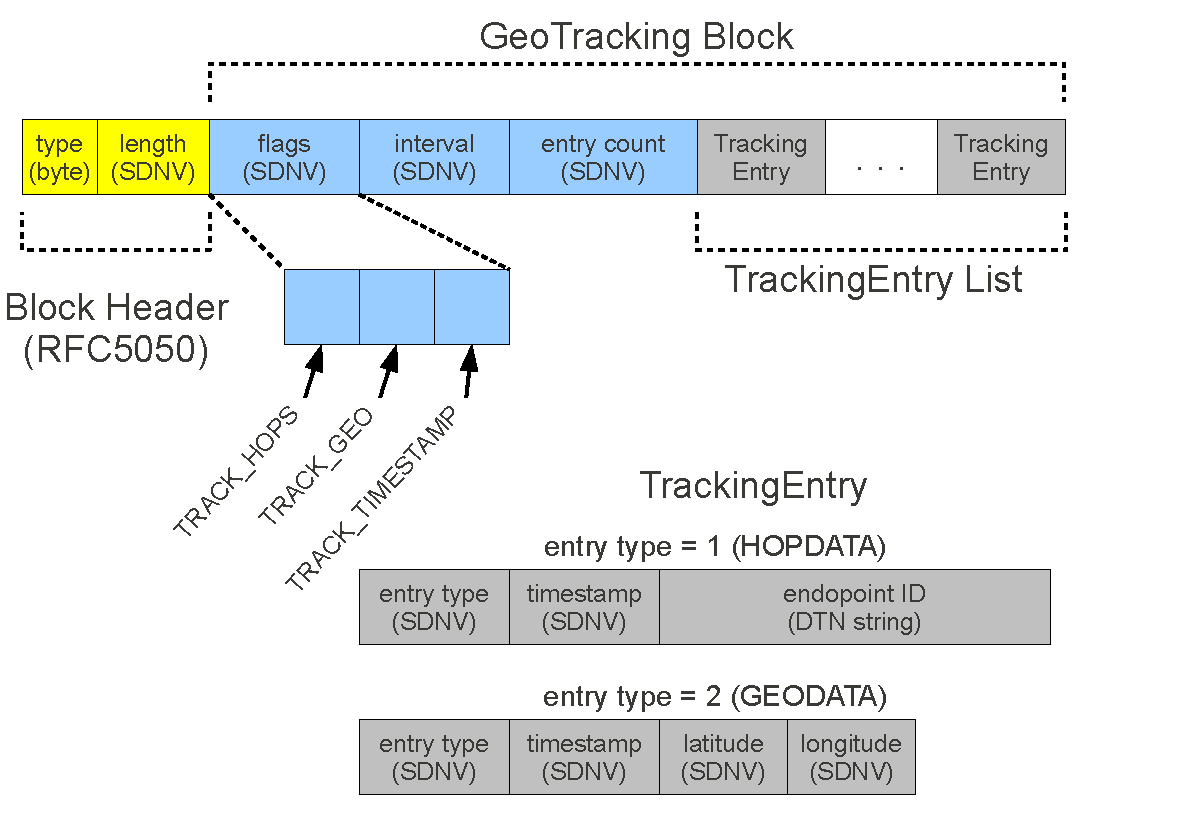
\includegraphics[width=\columnwidth]{figures/tracking-block.pdf}
\end{center}
\vspace{-.75cm}
\caption{Format of the GeoTracking Block}
\label{fig:tracking-block}
\vspace{-.5cm}
\end{figure}

\begin{sloppypar}
Figure~\ref{fig:tracking-block} depicts the {\em GeoTracking} block's format. The Block Header fields are specified by RFC5050\footnote{\scriptsize\url{http://tools.ietf.org/html/rfc5050}} and apply to any block in a bundle. In IBR-DTN, the block processor only deals with the contents of the block itself, and the BPA strips off the block header. Each {\em GeoTracking} block contains three mandatory fields:
\begin{description*}
  \item[Flags.] The flags tell intermediate BPAs what information to append to the block. The flags are: {\bf TRACK\_HOPS} (0x01), {\bf TRACK\_GEO} (0x02), and {\bf TRACK\_TIMESTAMP} (0x04).
  \item[Interval.] The interval (in seconds) tells intermediate BPAs the frequency with which to append a new GEODATA tracking entry to the entry list.  
  \item[Entry Count.] The entry count keeps track of the number of tracking entries contained in the block.
\end{description*}
\end{sloppypar}

Keeping each bundle's {\em GeoTracking} block updated as the device storing the bundle moves is non-trivial; keeping a {\em GeoTracking} block up-to-date in real time is not feasible for several reasons. First, there may be many bundles at a given BPA with {\em GeoTracking} blocks, and each bundle may have a different interval, requiring both responding to multiple timers and (in the case of IBR-DTN), reloading and storing each bundle from disk on every update. Instead, we maintain a global GPS log and updates a bundle's associated {\em GeoTracking} block only when a bundle is serialized for sending. Upon serialization, we examine the history of the GPS log and attach all of the appropriate entries to the {\em GeoTracking} block. Maintaining the GPS log is also non-trivial. To completely satisfy any arbitrary tracking interval requirement would require recording the node's location at an interval of the GCD of all of the tracking intervals, which may not be know {\em a priori}. In our prototype, we choose a fixed global interval, and bundles can request a {\em less frequent} update. Finally is the question of where to maintain the GPS log. A BPA should be as platform-independent as possible, while GPS information acquisition is quite platform-dependent. Therefore, we assume a host-specific agent that logs GPS data to a file at the aforementioned interval. Each time a {\em GeoTracking} block is serialized, the BPA scans the log file for the necessary entries and creates the necessary tracking entries for the {\em GeoTracking} block.

This approach still has some drawbacks, especially in IBR-DTN.  First, it requires opening and reading a (potentially long) log file each time a {\em GeoTracking} block is serialized.  Second, in IBR-DTN, because there is no function to "finalize" the contents of a block prior to serializing, the GPS log must be parsed twice: once when the block processor calculates the block's length, and again when the actual serialization takes place.  
%In IBR-DTN both the {\bf getLength()} and {\bf serialize()} functions are {\bf const}, so it is not possible to modify any fields of the GeoTracking block itself to cache the state of the block when {\bf getLength()} is called.  
This technically creates a race condition between these two calls, where the GPS log may get longer between the two functions.  Resolving these issues completely may require some modifications to the serialization process of IBR-DTN and is reserved for future work.

%\subsubsection{GPS Coordinate Representation as SDNV} \label{gps-representation}
Our extension blocks represent GPS coordinates in signed degrees format, where latitude ranges from $-90^{\circ}$ to $90^{\circ}$ and longitude ranges from $-180^{\circ}$ to $180^{\circ}$.  Both latitude and longitude are considered to be type {\bf float}.  However, since the self-delimiting numeric values (SDNVs)\footnote{\scriptsize\url{http://tools.ietf.org/html/draft-irtf-dtnrg-sdnv-09}} used in the bundle protocol cannot represent floating point numbers or negative values, we make two transformations to encode longitude and latitude in the{\em GeoTracking} block.  If $\theta<0$ we compute $\theta^{\prime}=\theta+360^{\circ}$.  Then we scale all coordinates up by a factor of $1048576$.  This gives us at least 20 bits of precision in both values, which is more than enough for meter-level resolution in the GPS coordinates.  When the blocks are received and deserialized, these transforms are reversed to give the original floating point values.






% -----------------------------------------------
%   GeoRouting Block
% -----------------------------------------------
% -----------------------------------------------
%   GeoRouting Block
% -----------------------------------------------
\subsection{The GeoRouting Block}
\begin{sloppypar}
The {\em GeoRouting} extension block supports source-routing based on either intermediate geographic waypoints, logical hops (EIDs), or both.  A {\em GeoRouting} block is essentially a list of geo-routing entries, each one specifying an intermediate routing goal. The {\em GeoRouting} block's format is shown in Figure~\ref{fig:georouting-block}; its main part contains only two fields: the flags (which are currently unused) and an entry count that specifies how many geo-routing entries follow.  Each geo-routing entry has several fields.  The flags specify the requirements and contents of the entry. The four flags are:
\begin{description*}
  \item[REQUIRED.] If set, then this entry {\it must} be satisfied for the bundle to be considered delivered.  Otherwise the entry is considered optional.
  \item[ORDERED.] If set, then this entry {\it must} be satisfied before any successive entries can be considered.  Otherwise an intermediate node can pop following entries off the list before this one is satisfied.
  \item[GEO\_PRESENT.] If set, this entry contains a latitude/longitude pair to be used as a routing waypoint.  To satisfy this entry, the bundle must visit a node that is within a specified margin of this coordinate.
  \item[EID\_PRESENT.] If set, this entry contains an EID.  To satisfy this entry, the bundle must, at some point, visit a node whose singleton EID matches the required EID.
\end{description*}
\end{sloppypar}

\begin{figure}
\begin{center}
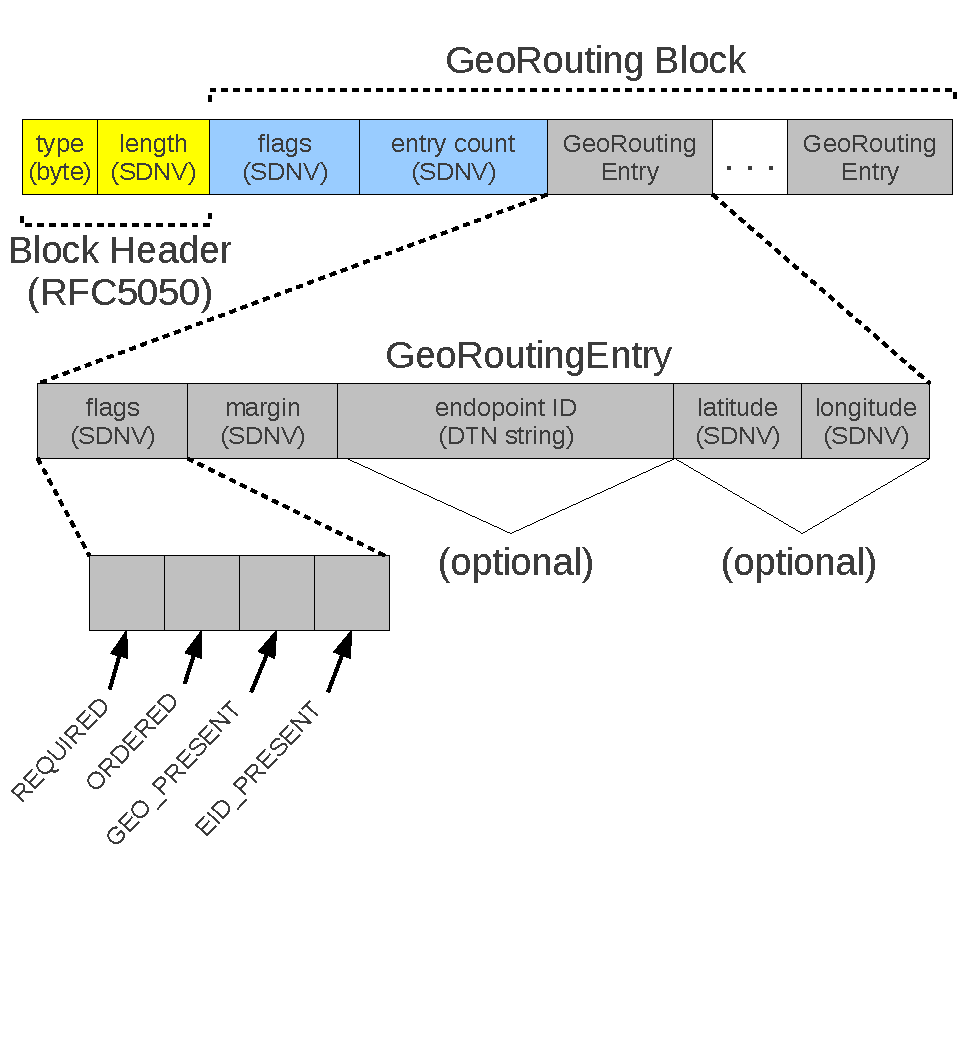
\includegraphics[width=.8\columnwidth]{figures/georouting-block.pdf}
\end{center}
\vspace{-.75cm}
\caption{Format of the GeoRouting Block}
\label{fig:georouting-block}
\vspace{-.5cm}
\end{figure}

If both {\bf GEO\_PRESENT} and {\bf EID\_PRESENT} are set, then the bundle must be carried by the node specified in the EID field to the location specified by the GPS coordinate.  {\bf REQUIRED} and {\bf ORDERED} could be set to false if the sender intends to allow the bundle to take a shortcut if one is available; some entries could be discarded if the bundle finds itself able to skip ahead in the specified geo-trajectory. Our router's use of these fields is described below.

The block's {\bf margin} specifies {\em how close} the block must come to each coordinate for the entry to be satisfied. The margin is given in absolute degrees. If $m$ is the margin and $x_0$ and $y_0$ are the required longitude and latitude, then getting the bundle within the range $(x_0\pm m, y_0\pm m)$ is sufficient.  This target area is roughly rectangular instead of circular, and a particular margin will result in different {\it actual} margins at different points on the globe.  Interpreting the margin as a radius in meters would require more complicated geodetic calculations each time a node's location changes. To represent the margin as an SDNV, we apply the same transformation as with GPS coordinates.

The {\em GeoRouting} block is easier to maintain for the block processor, but more complicated for the routing implementation. The details of these router updates are given in the next section. As with the {\em GeoTracking} extension block, we have implemented the {\em GeoRouting} block in both the IBR-DTN core and within the Java API; this allows Java-based applications to create geo-routed bundles directly.





% -----------------------------------------------
%   The Breadcrumb Router
% -----------------------------------------------
%\section{The {\sc breadcrumb} Router}
% -----------------------------------------------
%   The Breadcrumb Router
% -----------------------------------------------

The {\sc breadcrumb} router performs geo-source routing using the {\em GeoRouting} extension block, the location of the node, and the location of neighboring peers. When it receives a bundle with a {\em GeoRouting} block, the router examines the entry at the top of the list, and, if the entry contains a geo entry, the router compares the entry's location against its location and the locations of neighboring peers and decides whether it or a peer is within the specified margin of the required coordinate. If the router finds a match, it pops the top entry from the list stored on the {\em GeoRouting} block. The router also forwards bundles without popping entries in the {\em GeoRouting} block if it encounters a peer that is closer to the next required waypoint. %The name of this router comes from the fact that following these entries back to a particular location is analogous to following breadcrumbs.

The {\sc breadcrumb} router's functions are divided into three tasks in the IBR-DTN routing task-queue structure:
\begin{description*}
\item[SearchNextBundle.] Computes the next bundle to send to a peer; invoked when the router receives an event indicating a change in peer connectivity (e.g., a successful peer handshake or completed bundle transfer).
\item[UpdateMyLocation.] Updates the router's knowledge of the node's location; queued periodically and anytime a bundle is received.
\end{description*}

%{\bf Bundle Filters and Meta Bundles.}
{\bf SearchNextBundle} and {\bf UpdateMyLocation} both require inspecting the information in each bundle's {\em GeoRouting} block, which is challenging to do efficiently in IBR-DTN since bundles are kept in persistent storage. On the other hand, maintaining a data structure in memory that contains all the geo information for each bundle is counter to the design of IBR-DTN. We devised a solution that does not require creating an additional data-structure and minimizes the retrieval of bundles from persistent storage.  We rely on two IBR-DTN constructs: {\sc bundle filters} and {\sc meta bundles}. {\sc Meta bundles} are light-weight bundle representations that contain fields of particular interest. {\sc Bundle filters} query the storage for meta bundles that meet a set of criteria. We added three fields to the {\sc meta bundle}:
\begin{description*}
\item[hasgeoroute.] A boolean identifier indicating that the bundle has a {\sc GeoRouting} block.
\item[nextgeohop.] The last entry in the {\sc GeoRouting} block.
\item[reacheddest.] A boolean flag indicating that there are no more entries in the {\sc GeoRouting} block (i.e., the bundle has reached its ``final'' destination)
\end{description*}

We also created two {\sc bundle filters}, one pertaining to each task that needs to inspect the bundles:
\begin{description*}
\item[SearchNext.] Determines which bundles to send to each peer; invoked during {\sc SearchNextBundle}. For each {\sc meta bundle} for which {\sc hasgeoroute} is {\sc true}, the filter compares the location of each peer with the {\sc nextgeohop} to see if the peer is closer to it than the host. If so, the meta bundle is added to the list.
\item[UpdateLocation.] Determines which {\sc GeoRouting} blocks need updating; the decision is based on whether the location of the node is within the specified margin of error of the {\sc nextgeohop} from the meta bundle.
\end{description*}
Forwarding a bundle does not necessarily pop a geo entry off of the {\em GeoRouting} block; the {\sc breadcrumb} router also greedily forwards bundles to nodes that are {\em closer} to the next geo waypoint, even if they are not within the specified margin of error of the waypoint.

By using the {\sc bundle filters}, only one lookup into the persistent storage is required; it retrieves a list of {\sc meta bundles} that need action. For {\sc SearchNextBundle}, the {\sc meta bundles} contain the information necessary to determine which bundles to transfer. For {\sc UpdateMyLocation}, each {\sc meta bundle} represents a bundle that needs to be pulled from persistent storage to have its {\em GeoRouting} block updated. 
%The filter limits this retrieval to exactly the bundles that need to have their list of geo-routing entries updated (i.e., by having a satisfied entry popped from the list). 
This is a considerable improvement over retrieving every bundle just to inspect a {\em GeoRouting} block that, in the majority of cases, will not require updating.

The {\sc breadcrumb} router defaults to epidemic routing when bundles do not contain {\sc GeoRouting} blocks. We can therefore use a single router to build trajectories using {\em GeoTracking} blocks (i.e., to drop breadcrumbs) and to use {\em GeoRouting} blocks to return to the source (i.e., to follow breadcrumbs). The router supports single-copy routing, so that only a single copy of the bundle with a {\em GeoRouting} block persists in the network. For our prototype, the router provides ordered, geo-source routing, i.e., it assumes that all {\em GeoRouting} blocks contain entries that must be visited in order, and that each entry pertains to a particular geo location. Our {\em GeoTracking} and {\em GeoRouting} extension blocks apply more widely; supporting a heterogeneous series of entries would make the router more generalizable since it could be applied to scenarios where the order that locations are visited does not matter, or where a few specific nodes must be visited.

%Although not specifically associated with our router, current IBR-DTN does not support updates to bundles in storage. Therefore, each update to a {\sc GeoRouting} block requires a separate remove and store operation. This is inefficient because it requires that the entire bundle be re-written to storage during every update (this actually makes our modifications to the meta bundles even more critical). Adding this update functionality would improve the performance of our router and of IBR-DTN storage in general.




% -----------------------------------------------
%
%   Experiments
%
% -----------------------------------------------
\section{Experiments}\label{sec:experiments}
To demonstrate and evaluate our GeoTracking and GeoRouting, 
we integrated these extensions with the IBRDTN implementation, and performed experiments on 
the VMT channel-emulated testbed~\cite{hahn10:using, kim11:reality}.  

\subsection{VMT Testbed Results}\label{sec:vmtresults}
We ran several experiments on the VirtualMeshTest (VMT)
mobile wireless testbed~\cite{hahn10:using, kim11:reality}.
VMT allows us to subject Linux-based real wireless nodes with commodity 
wireless hardware to emulated mobile environments.  The 
wireless testbed is effectively an analog channel emulator based
on an array of programmable attenuators.  Given a desired physical arrangement
of nodes, the system computes the expected path loss between
nodes and programs the attenuators to achieve those path loss
properties.  By updating the attenuations every second, VMT can
emulate a mobile wireless environment for real wireless nodes.

\subsection{Crop Circles Scenario}



\begin{figure}
\vspace{-.2cm}
\begin{center}
%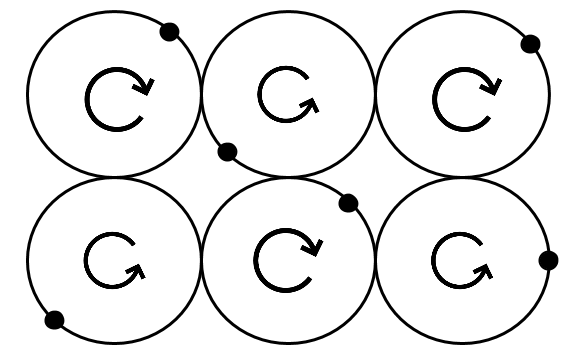
\includegraphics[width=\columnwidth+.5]{figures/cropcircle1.png}
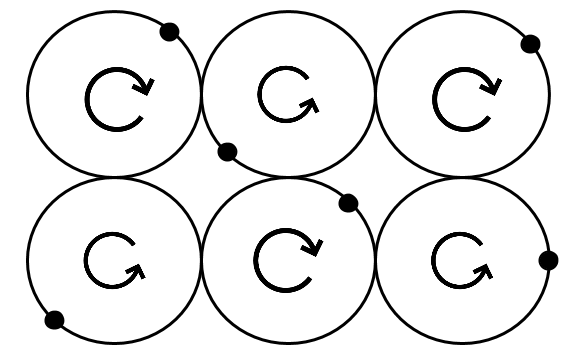
\includegraphics[width=3in]{figures/cropcircle1.png}
\end{center}
\vspace{-.4cm}
\caption{Crop Circles Experiment}\label{fig:cropcircle1}
\vspace{-.35cm}
\end{figure}

The first crop circles mobility scenario consists of six mobile nodes, arranged in two rows. As shown in 
Figure~\ref{fig:cropcircle1}, some nodes follow a circle in a clockwise direction, and some nodes follow a counter-clockwise path. The source in these experiments is the lower left node, and the responder is the upper right node.



%The second crop circles mobility scenario, shown in Figure~\ref{fig:cropcircles2}, consists of eighteen mobile nodes, arranged in six rows. The source in these experiments is Node 1, and the responder is Node 18.




% -----------------------------------------------
%
%   Conclusion
%
% -----------------------------------------------
\section{Conclusion}




% Once the sections and outline are solidified, breaking the paper up into separate files will be useful.  For now I'll put the sections inline.
%
%% -----------------------------------------------
%
%   Introduction
%
% -----------------------------------------------
\section{Introduction}
Applications in delay-tolerant networks (DTNs) often desire to both track the path(s) of data through the network and to directly influence the movement of the data. DTNs are almost always integrated into some physical space that also influences that movement of nodes, data, and the phenomena about which the nodes communicate. In traditional IP networks, the {\bf traceroute} tool and {\bf source routing} protocols have assisted in {\em tracking} and {\em directing} packets of data, but the focus has traditionally been on movement through the logical network and not through physical space.

When the physical and logical intertwine, there is a desire for data movement to reflect various aspects of the physical space the data inhabits. We address the dual challenges of {\em tracking} data as it moves through space and time and intentionally {\em routing} data through space and time. As an exemplar of tracking, consider the need for {\em data provenance} in sensing aggregation. As an aggregate collects information sensed about a physical phenomenon, the aggregate may need to dynamically compute the data {\em coverage} by tracking where the aggregate has traveled and collected information~\cite{michel12:spatiotemporal}. As an exemplar of the routing challenge, consider a piece of data that measures the concentration of a gas leak. Users in the area where the gas is expected to dissipate should be warned; this can be accomplished by associating the data item with a route through space and time that captures this expected dissipation. Tracking and routing can also be combined; imagine a generic scenario in which a {\em publisher} generates a piece of data that tracks its movement {\em en route} to a {\em subscriber}. Upon receiving the publication, the subscriber sends a response that must follow the reverse path of the original publication. This generic situation is a stand-in for a variety of concrete applications. For example, the original publication may have reserved some resources along the routing path that the return response relies on. In the later sections of this paper, we use a concrete story behind this more general scenario. Specifically, we consider a maze traversal in which a prisoner in the maze sends a probe that tracks its path as it attempts to exit the maze. When it reaches the exit, the responder (e.g. a rescuer) sends a response packet back to the prisoner along the same path through the maze.

Our problem of tracking differs substantially from the goals of existing utilities, not only in terms of the transition from logical network hops to physical spaces but also because the route a bundle in a DTN takes may not be stable (one bundle may pass through a given sequence of nodes, while a bundle sent just a minute later may take a different route). It therefore may often be important to track the route of {\em each} bundle. In our tracking facility, we track {\em both} logical network hops and the sequence of geographic locations it visits (whether because a device at one location transmits the bundle to a device at a different location or because the device holding the bundle moves). Besides being an illuminating diagnostic tool to understand the behavior of a DTN, tracking a bundle's geographic route can capture important meta-information related to the bundle's contents, as motivated above. 

Source routing, in which a packet carries with it the specific network hops it must traverse, and geographic routing, where packet routing is based on physical locations, have been popular in mobile ad hoc networks~\cite{johnson96:dynamic, karp00:gpsr}. We combine these approaches into a geographically informed version of source routing. Previous approaches to geographic routing predominantly use a {\em greedy} approach in which locally optimal decisions are used to move a bundle incrementally closer to its destination. Our approach to {\em geo-source routing} differs in that it allows the sender to pre-specify a sequence of geo-locations that serve as routing {\em waypoints}. This style of approach can solve a variety of challenges associated with traditional geographic routing. For example by explicitly directing the geographic path of a bundle, our protocol can explicitly route around known dead-ends in the network or around known areas of congestion in the network. Combining this style of geo-routing with other approaches could, for example, ensure that network coded bundles~\cite{petz11:network, widmer05:network} take sufficiently diverse routes through the network.

We introduce the {\sc breadcrumb} router, which implements geo-source routing on DTN bundles that can pre-specify their own delivery paths by providing a combination of geo-locations and logical network hops. 
%In our {\sc breadcrumb} router, elements in this sequence can be {\em required}, meaning that the bundle must touch the specified logical or physical location or {\em optional}, meaning that the sequence serves as a suggestion that the {\sc breadcrumb} router can use simply to guide its decision making. 
Each geo-location comes with a {\em margin of error}, which allows the bundle to get {\em near} the specified location without having to exactly reach it. We also introduce two bundle {\em extension blocks}. The {\em GeoRouting} block holds the sequence of logical and geographical waypoints for geo-source routing. The {\em GeoTracking} block allows any bundle to collect a sequence of locations it visits in both logical and physical space. In our implementation, we rely on a GPS module to provide location information. Throughout the paper, we use the phrases ``GPS location'' or ``GPS coordinates'' to refer to this information, but we note that the GPS framework is a stand-in for any available, potentially highly fine-grained location service framework.  We describe our the {\sc breadcrumb} router and the two extension blocks conceptually and show how we have implemented them in the IBR-DTN implementation of the bundle routing protocol~\cite{IBR-DTN-WASA}. We connect the {\sc breadcrumb} router to our existing Java-based implementation of {\em spatiotemporal trajectories}~\cite{michel12:spatiotemporal}, in which applications can perform expressive computations over data items given knowledge of their movements in space and time and geo-tracking and geo-routing of bundles on a pair of mobility scenarios.



%{\color{blue}
%Since the dawn of time, man has wanted to know where the heck his bundles went, and to send them back on a specific geo-coded route.  Our new BreadCrumb Router and its associated extension block processors satisfy this cosmic desire of human existence.  

%The {\bf traceroute} tool is a staple of traditional IP networks.  It allows a user or administrator to discover the sequence of IP routers their packets pass through between a specific source and destination.  Traceroute works by taking advantage of existing IGMP hop-count and reporting requirements.  Bundle Protocol as defined in RFC5050 has no inherent facility that can achieve this.  Furthermore, because the route a bundle takes may not be stable (one bundle may pass through one sequence of nodes, and a bundle sent a minute later may take another route) it is more salient in a DTN to comprehensively track the entire route of a single bundle, rather than send a series of bundles to probe the network.  Therefore bundle tracking functionality must be built fully as an extension to BP.  Additionally, since in many use cases the geographic mobility of the nodes in a DTN plays an integral part in the routing and delivery of a bundle, tracking the geographic route a bundle follows can be at least as interesting, and possibly {\it more} salient than the logical hops the bundle passes through.

%Besides being an illuminating diagnostic tool to understand the behavior of a DTN, tracking the geographic route of a bundle can capture important meta-information related to the contents of a bundle.  The simplest example of this is simply geo-tagging the location where a bundle originated.  A more involved example is tinkerpopping the datums of an oil slick with trajectories with a graph database as described in \cite{jonas-paper} and to be elaborated on here and in the following sections by Jonas and Christine.  Datums: it's the plural of ``datum'' when you're talking about geodetic information, dammit!

%Converse to simply geotracking a bundle, we build a prototype router for source geo-routing of a bundle.  In traditional IP networks, extensions to support source routing are defined for both IPv4 and IPv6, but are rarely used and often not supported or blocked.  On the other hand source routing is an integral part of some MANET routing protocols \cite{some-DSR-paper}.  Some reasons source routing could be used are to probe the structure of a network, or to specify that packets should avoid sections of a network that are known to be problematic because of congestion, reliability, or security concerns.  Implementing this type of {\it logical} hop-based source routing in DTN is certainly feasible, but in a dynamic mobile network is is difficult to imagine that a source will know exactly which intermediate nodes will be available to ferry its bundles.  Considering the importance of the geographic path in DTN routing, we propose geographic source routing.  In this system a sender can specify both logical (intermediate nodes) and geographic waypoints a bundle must pass through on its way to the destination.

%Geographic routing has been proposed and used in many DTN scenarios \cite{paper1,paper2,paper3,paper4,paper5,paper6}.  In most cases greedy geographic routing is used locally to move a bundle closer to a destination.  In other cases large-scale logical hops over an infrastructure network are used to get a bundle to a general geographic area of interest, and then other types of routing take precedence to get the bundle to its final destination.  Source geo-routing is different in that it allows a sender to pre-specify solutions to problems that can arise from greedy geographic routing.  Some of these issues and goals are:
%\begin{itemize}
%  \item avoiding known dead-ends in the network. I.e. local minima in the greedy geographic routing heuristic.
%  \item avoiding geographic areas where unreliability or congestion is anticipated.  For example if a shortest geographic route goes past a baseball stadium, but a game is scheduled for that day, a source may request that a bundle be routed around the expected traffic jam.
%  \item ensuring that network coded bundles take sufficiently diverse routes.  Since network coded information can be viewed as a shared secret problem, ensuring that not all of the encodings are ever in the same geographic area could be a security measure in a DTN.
%\end{itemize}
%\footnote{Brenton's original text, a lot of which gets reused in the above structure}
%}
%\input{background}
%\input{routing}
%\input{evaluationPharos}
%\input{evaluationNYC}
%\input{evaluationVMT}
%\input{evaluationBrief}
%\input{conclusion}
%\input{related}
% removed in favor of combining related work with "Background" section
%\section*{Acknowledgments}
%This work was funded in part by the US Dept. of Defense. The views expressed are those of the authors and may not necessarily reflect the views of the sponsoring agencies.\\

\bibliographystyle{abbrv}
%\begin{scriptsize}
\bibliography{cjbib}
%\end{scriptsize}

\end{document}

